\documentclass{beamer}
\usepackage[utf8]{inputenc}
\usepackage{listings}
\usepackage{booktabs}
\usepackage{bm}
\usepackage{enumitem}
\usepackage[export]{adjustbox}
\usepackage{svg}

\usetheme{Madrid}
\definecolor{mlpblue}{rgb}{0.1, 0.14, 0.24}

\useoutertheme{infolines} % Alternatively: miniframes, infolines, split
\useinnertheme{circles}
\usecolortheme[named=mlpblue]{structure}

\lstset{basicstyle=\footnotesize\ttfamily,breaklines=true}

%------------------------------------------------------------
%This block of code defines the information to appear in the
%Title page
\title[G-Transformation Invaraiance]{Neural Networks for Learning Counterfactual G-Invariances from Single Environments}

\subtitle{``Fixing the Image Rotation Problem''}

\author[Machine Learning @ Purdue] % optional
{J.~Setpal} 

\date{\today}

\titlegraphic{
\includegraphics[width=7cm]{../shared/logo-long.pdf}}

%End of title page configuration block
%------------------------------------------------------------

%The next block of commands puts the table of contents at the 
%beginning of each section and highlights the current section:

\AtBeginSection[]
{
  \begin{frame}
    \frametitle{Outline}
    \tableofcontents[currentsection]
  \end{frame}
}
% ------------------------------------------------------------


\begin{document}

%The next statement creates the title page.
\frame{\titlepage}

\begin{frame}
\frametitle{Outline}
\tableofcontents
\end{frame}

%% motivations
%% invariances / equivariances in CNNs
%% group theory background
%% obtaining g-invariance
%% obtaining g-equivariance

\section{Motivation}
\begin{frame}{Introduction}
	Convolutional Neural Networks are \textit{fantastic}. They efficiently extract a vast range of relevant contextual features and are resistant to pixel shift.

	\begin{center}
		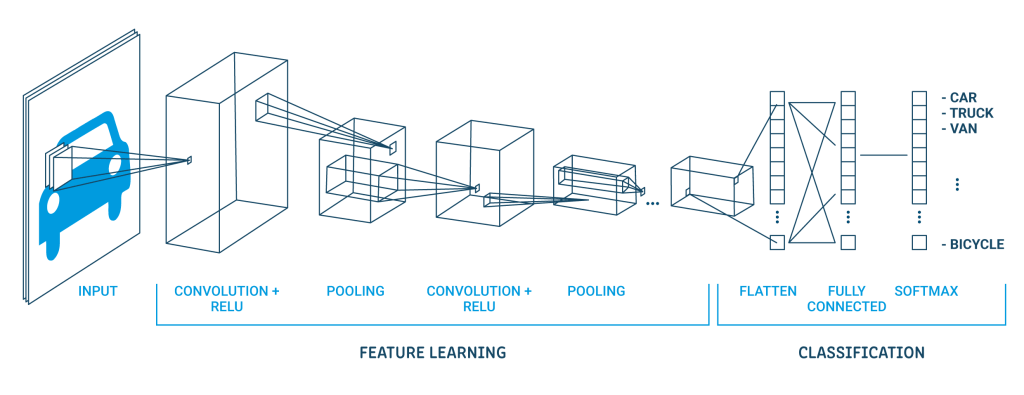
\includegraphics[width=\textwidth]{img/cnn.png}
	\end{center}

	\pause
	However, they have a \textbf{critical flaw}.
\end{frame}

\begin{frame}{Neural Networks Aren't Rotationally Robust.}
	\textbf{Q}${}_1$: Do you think that a CNN trained on a distribution of the left image \textit{should} classify the right image as the same class for each of these pairs?
	\vspace{-.9em}
	\begin{center}
		
\includegraphics[width=\textwidth]{img/rot.png}
	\end{center} 
	\pause
	\vspace{-1em}
	\textbf{A}${}_1$: Definitely! \pause \newline \\
	\textbf{Q}${}_2$: In practice, does this actually happen? \pause \\
	\textbf{A}${}_2$: Nope -- all these images were misclassified. \pause \newline \\
	\textbf{Q}${}_3$: How can we fix this? \pause \\
	\textbf{A}${}_3$: Data Augmentation (boring)\pause, \textbf{G-Invariant Transformations} (fun)!
\end{frame}

\section{Set Theory}
\begin{frame}{Understanding Groups}
	\textbf{Definition:} A group is a set $G$, with an operator $\odot$ that acts on $\forall g_1, g_2 \in G$. \pause $(G, \odot)$ has the following properties:
	\begin{enumerate}[label=\alph*.]
		\item It's closed under combination. $g_1 \odot g_2 = g_3 \in G$ \pause
		\item It contains an identity. $\exists I \in G$ s.t. $g_1 \odot I = g_1\ \forall g_1 \in G$ \pause
		\item It contains an inverse. $\exists g_1^{-1} \in G$ s.t. $g_1 \odot g_1^{-1} = g_1^{-1} \odot g_1 = I$ \pause
		\item $\odot$ is associative. $g_1 \odot (g_2 \odot g_3) = (g_1 \odot g_2) \odot g_3$ \pause
		\item (Optional) $\odot$ is commutative (abelian). $g_1 \odot g_2 = g_2 \odot g_1$ \pause
		\item (Optional) Can be finite ($|G| < \infty$) or infinite ($|G| = \infty$). \pause
	\end{enumerate}
	~\\

	\textbf{Q:} Why do we care? \pause \\
	\textbf{A:} We leverage \underline{axioms a-d} to derive a \textbf{transformation invariant representation} of our input. Invariance holds iff axioms a-d also hold.
\end{frame}

\begin{frame}{The General Linear Group}
	A linear transformation is defined as: 
	\begin{gather}
		T(v) = Av \text{ where } v \in \mathbb{R}^n,\ A \in \mathbb{R}^{m \times n},\ T: \mathbb{R}^{n} \rightarrow \mathbb{R}^m
	\end{gather} \pause
	If $A \in G$ is a linear transformation, $G$ is a \textbf{linear group}. \pause \newline \\

	The \textbf{general linear group} is the set of all invertible transformations:
	\begin{gather}
		GL_n: (M_{n \times n}(\mathbb{R}), \odot)
	\end{gather} \pause
	Next, we define general linear groups over some affine transformations.
\end{frame}

\begin{frame}{GL Tranformation Groups over Images}
	Let our input $x \in \mathbb{R}^{3 \times n \times n}$ be our input image. Consider $\text{vec}(x) \in \mathbb{R}^{3n^2}$. \pause
	\begin{gather}
		G_{rot} \equiv \{T^{0^\circ}, T^{90^\circ}, T^{180^\circ}, T^{270^\circ}\} \\
		G_{flip} \equiv \{T^{v}, T^{h}, T^{180^\circ}, T^{0^\circ}\}
	\end{gather} \pause
	\vspace{-2em}
	\begin{center}
		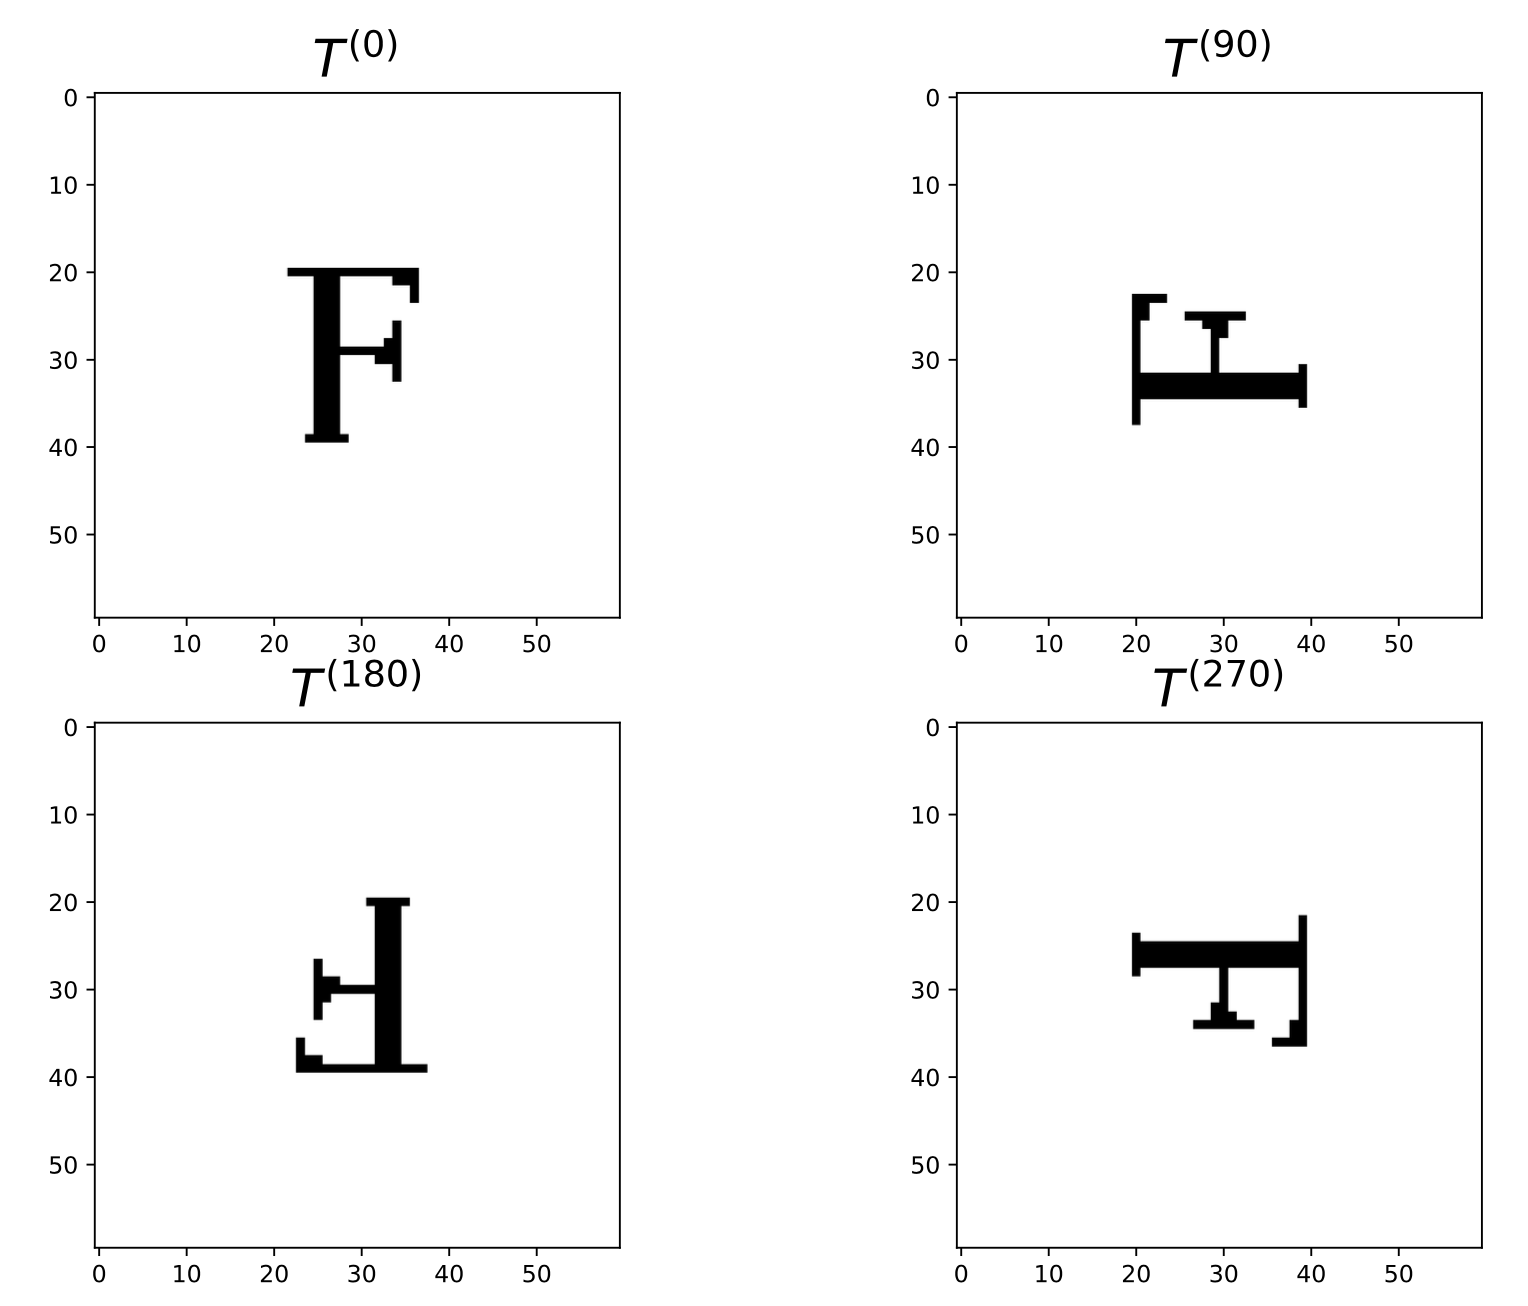
\includegraphics[width=0.5\textwidth]{img/f_rots.png}
	\end{center} \pause
	Both groups are defined over $G: \mathbb{R}^{3n^2} \rightarrow \mathbb{R}^{3n^2}$
\end{frame}

\section{Leveraging Set Theory (Fun Part)}
\begin{frame}{Obtaining an Invariant Transformation}
	Defining the transformations as a \textbf{group} gives us \textit{guarantees} we can exploit to ensure \textbf{invariance} to those transformations. \pause \newline \\

	Formally, we want to make our input image invariant to rotation:
	\begin{gather}
		\forall T,\ \bar{T}(\bm{T}x) = \bar{T}x \text{ where } \bm{T} \in G_{rot}
	\end{gather} \pause
	We can integrate this into the definition of a nueron:
	\begin{gather}
		\sigma(w^Tx + b) \stackrel{def}{=} \sigma(w^T \bm{T} x + b)
	\end{gather} \pause
	\textbf{Lemma:} We can find $\bar{T}$ using the \textit{Reynold's Operator}.
	\begin{gather}
		\bar{T} = \frac{1}{|G|}\sum_{g \in G}g
	\end{gather} \pause
	Now, we have $\bar{T}$ s.t. $\bar{T} \circ T = T$!
\end{frame}

\begin{frame}{Invariant Subspace of $\bar{T}$}
	Now, we need to find $M \subseteq \mathbb{R}^d$ s.t. $\forall w^T \in M,\ w^T \bar{T} \in M$. \pause \newline \\

	One example of an invariant subspace is the left-1 eigenspace of $\bar{T}$:
	\begin{gather}
		\text{Left-1-Eig}(\bar{T}) = \{ w \in \mathbb{R}^d\ |\ w_T\bar{T} = w^T \}
	\end{gather} \pause
	Extracting those eigenvectors, we get $V = \{\bm{v}_i \}^k_{i=1}$ s.t. $\forall \bm{v}_i \in V$:
	\begin{gather}
		\bm{v}_i^T \bar{T} = \lambda_i \bm{v}_i
	\end{gather}
	By definition of eigenvectors. \pause \newline \\

	Since $\bar{T}$ is a projection operator, $\lambda_i = 1\ \forall i$:
	\begin{gather}
		\bm{v}_i^T \bar{T} = \bm{v}_i
	\end{gather}
\end{frame}

\begin{frame}{Putting it All Together}
	We can use our invariant bases $V = \{\bm{v}_i \}^k_{i=1}$ to create an invariant layer.
	\begin{gather}
		w^T = \sum^k_{i=1} w_i \bm{v}_i
	\end{gather} \pause
	Finally, we construct our group invariant layer:
	\begin{gather}
		h_{inv} = \sigma(w^Tx + b) = \sigma(w^T T x + b)\ \forall T \in G_{rot}
	\end{gather} \pause
	From here, the rest of the MLP follows the standard definition.
\end{frame}

\begin{frame}{Equivariance for CNNs}
	Our previous approach leveraged an isomorphism, which requires $\mathbb{R}^n \rightarrow \mathbb{R}^n$. This fails to hold for CNNs. \pause \newline \\

	Instead, a more relevant property we can investigate is equivariance:
	\begin{gather}
		\rho_1(g) W x = W \rho_2(g) x;\ g \in G, \rho_1: G \rightarrow \mathbb{R}^{n \times n},\ \rho_2: G \rightarrow \mathbb{R}^{k \times k}
	\end{gather} \pause
	Since this holds over our entire input $x$, we can re-arrange it as:
	\begin{gather}
		\rho_1(g) W \rho_2(g)^{-1} = W
	\end{gather} \pause
	This can be re-arranged to demonstrate an equivalency with \textit{invariance}:
	\begin{gather}
		\underbrace{\rho_2(g) \times \rho_1(g^{-1})^T}_{\bar{T}} \underbrace{\text{vec}(W)}_x = \underbrace{\text{vec}(W)}_x
	\end{gather} \pause
	From there, the previous invariance proof follows.
\end{frame}

\begin{frame}{Let's Demonstrate!}
	Here's what the final architecture looks like:
	\begin{center}
		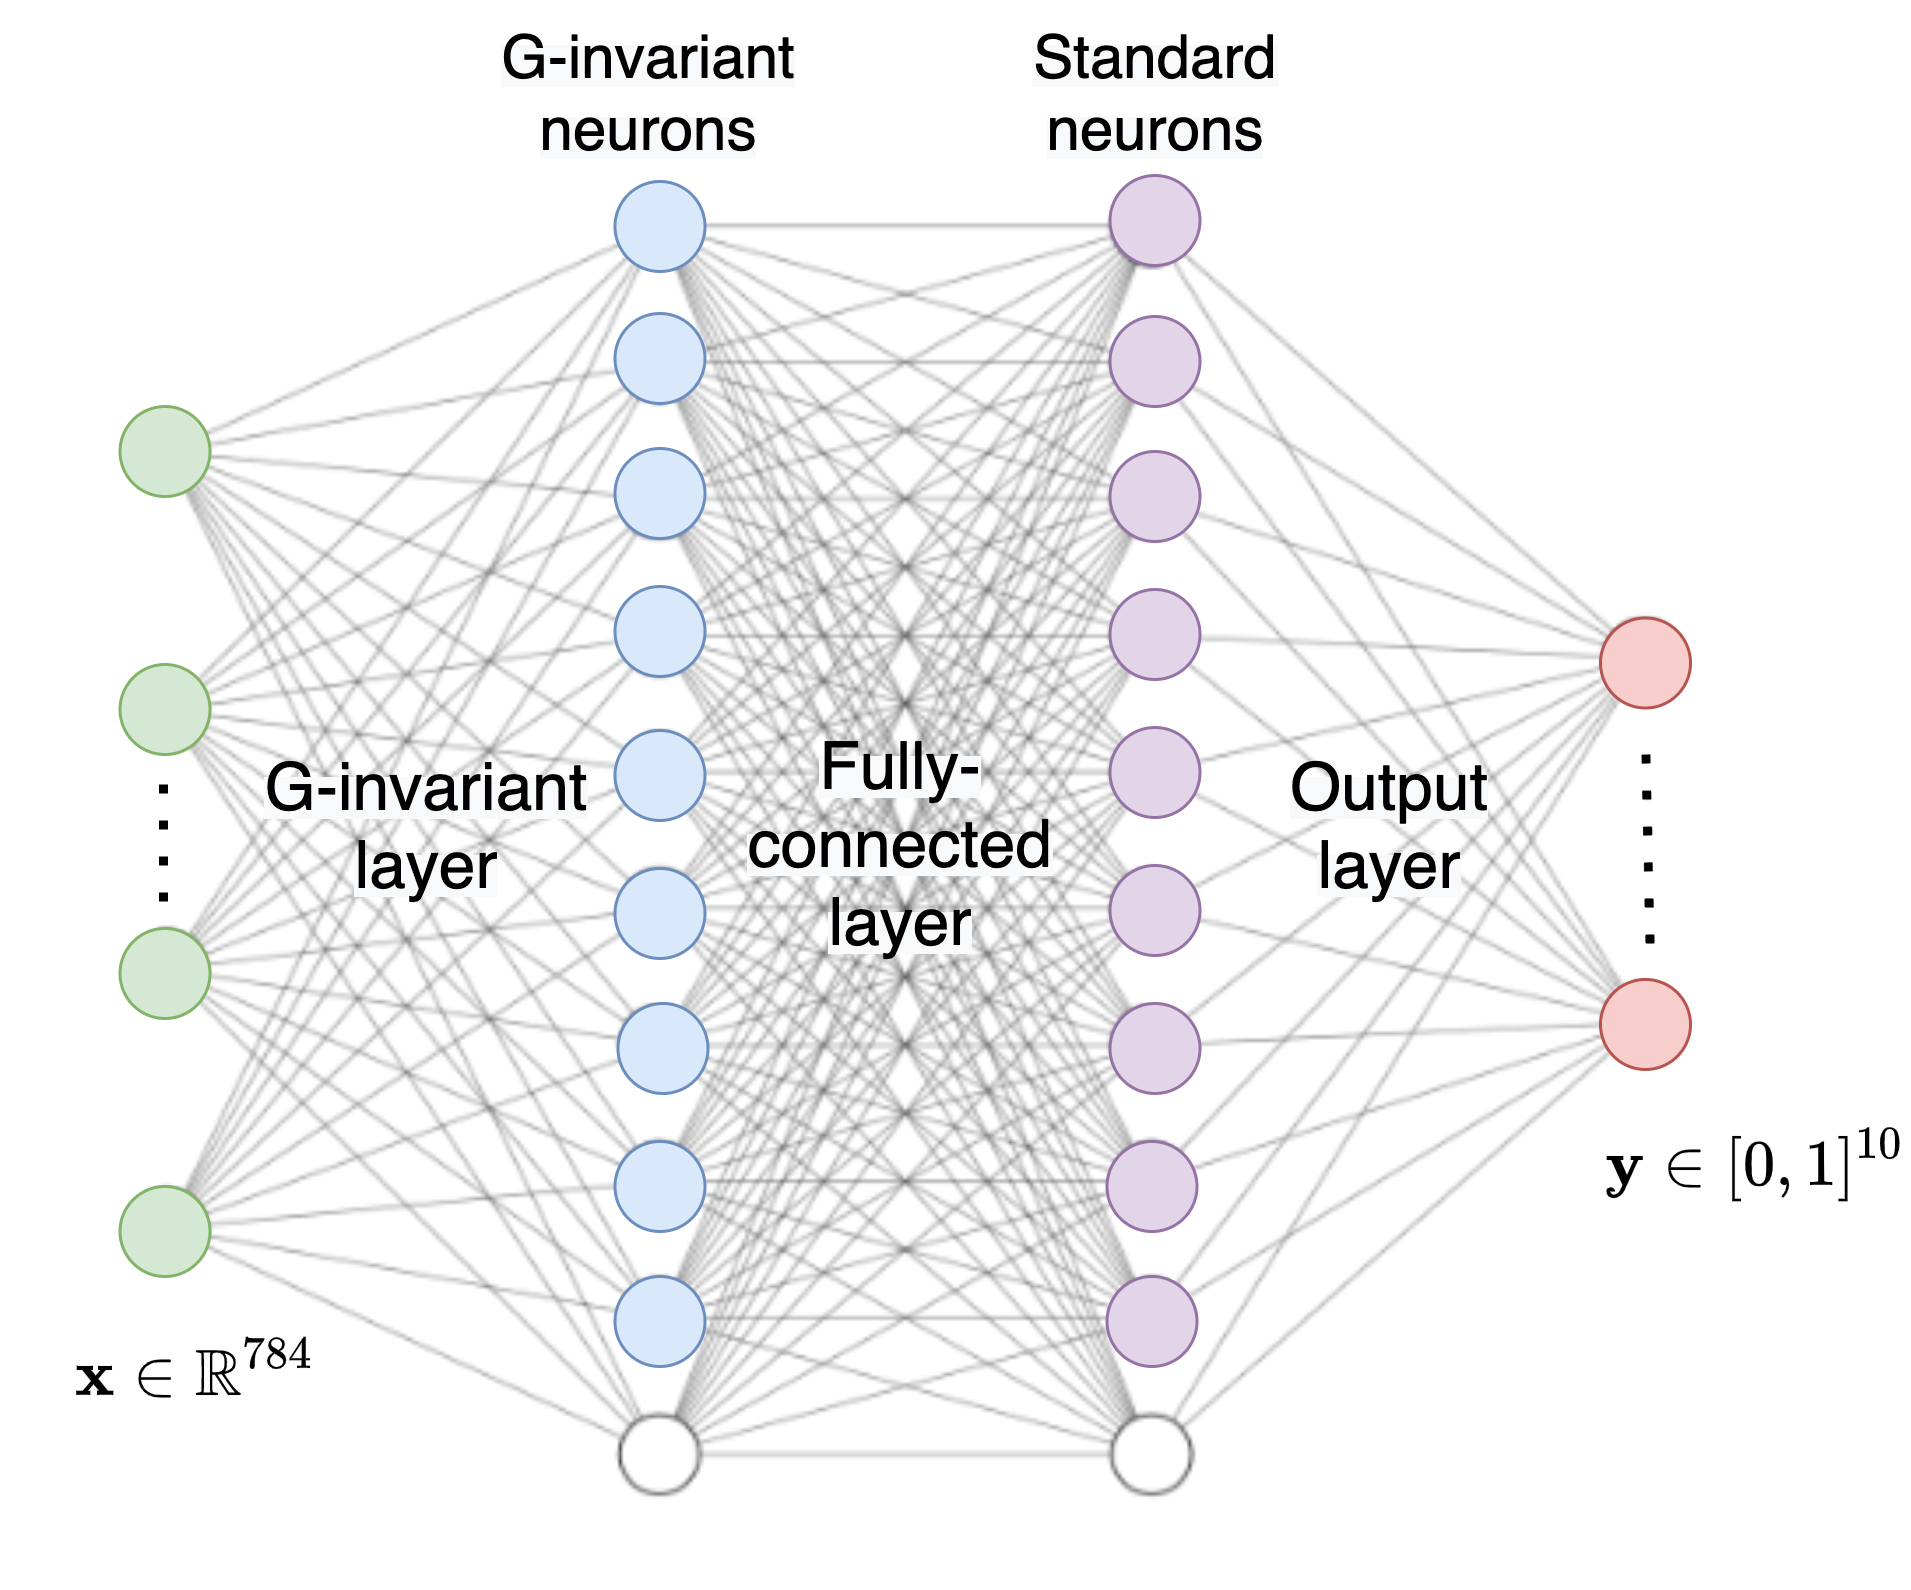
\includegraphics[width=.7\textwidth]{img/mlp.png}
	\end{center}
\end{frame}

\begin{frame}{Thank you!}
	\begin{center}
		Have an awesome rest of your day!
	\end{center}
	\begin{align*}
		\textbf{\small Paper:}&~\texttt{\small\url{https://arxiv.org/abs/2104.10105/}} \\
		\textbf{\small Slides:}&~\texttt{\small\url{https://cs.purdue.edu/homes/jsetpal/slides/gti.pdf}} \\
		\textbf{\small Notebook:}&~\texttt{\small\url{https://cs.purdue.edu/homes/jsetpal/nb/gti.ipynb}} \\
	\end{align*}
\end{frame}

\end{document}
